\documentclass{scrreprt}
\usepackage[french]{babel}
\usepackage[utf8]{inputenc}
\usepackage[usenames,dvipsnames]{color}
\usepackage{listings}
\usepackage{underscore}
\usepackage[bookmarks=true]{hyperref}
\usepackage[]{graphicx}
\DeclareGraphicsExtensions{.pdf,.png,.jpg}
\lstset{language=xml,frame=single, breaklines=true, basicstyle=\ttfamily,backgroundcolor=\color{white},basicstyle=\scriptsize, keywordstyle=\color{blue}, commentstyle=\color{Gray}, stringstyle=\color{red}, identifierstyle=\color{green}}

%%%% debut macro %%%%
\newenvironment{changemargin}[2]{\begin{list}{}{%
\setlength{\topsep}{0pt}%
\setlength{\leftmargin}{0pt}%
\setlength{\rightmargin}{0pt}%
\setlength{\listparindent}{\parindent}%
\setlength{\itemindent}{\parindent}%
\setlength{\parsep}{0pt plus 1pt}%
\addtolength{\leftmargin}{#1}%
\addtolength{\rightmargin}{#2}%
}\item }{\end{list}}
%%%% fin macro %%%%

\hypersetup{
    bookmarks=false, % show bookmarks bar?
    pdftitle={Projet SASIAE}, % title
    pdfauthor={Raynal Jean-Raymond, Dauphin Loïc, Clément Lansmarie, Hugo Brunie, Nicolas Belin, Benoit Gilbert, Théotime Méralli-Ballou}, % author
    pdfsubject={TeX and LaTeX}, % subject of the document
    pdfkeywords={TeX, LaTeX, graphics, images}, % list of keywords
    colorlinks=true, % false: boxed links; true: colored links
    linkcolor=blue, % color of internal links
    citecolor=black, % color of links to bibliography
    filecolor=black, % color of file links
    urlcolor=purple, % color of external links
    linktoc=page % only page is linked
}%1 
\def\myversion{}
\title{
\flushright
\rule{16cm}{5pt}
\vskip1cm
{\Huge Projet SASIAE}\\
\vspace{10cm}
{\small Théotime Méralli-Ballou\\ Jean-Raymond Raynal\\ Clément Lansmarie\\ Benoit Gilbert\\ Loïc Dauphin\\ Nicolas Belin\\ Hugo Brunie\\ }
\vfill
\rule{16cm}{5pt}
}
\date{}
\usepackage{hyperref}

\begin{document}

\maketitle
\tableofcontents

\chapter{Introduction}
% HUGO
Le but d'un simulateur de robot est de tester un robot et donc son code, sans nécessairement l'avoir construit. Un simulateur de robot doit aussi permettre de vérifier que le comportement du robot dans un environnement 3D correspond bien à ce qui était imaginé au départ. Eirbot est une association qui conçoit des robots pour participer à la coupe de France de robotique. Celle-ci consiste à opposer de deux à quatre robots autonomes qui interagissent avec les différents objets sur une table dans le but de marquer un maximum de points. L'association a besoin de fiabiliser ses robots, via plus de tests et une meilleure compréhension de leur comportement. Un simulateur permettra de mieux comprendre l'enchainement du code et ainsi de cibler les erreurs d'exécution plus rapidement qu'une mise en scéne réelle.

% (Loïc) Beaucoup de "robot" dans ce paragraphe... J'en ai retiré un peu.

%% TODO : Préciser qu'EIBROT utilise des AVR plutôt dans la partie existant 

\section{Objectifs}

%Hugo
Nous avons un double objectif pour ce projet. Dans un premier temps nous devons concevoir et implémenter une API, Aversive++, qui fera l'interface entre le code robot et le simulateur. En même temps, nous devons développer un simulateur capable de reproduire une situation de jeu et interagir avec le code robot, à travers Aversive++. Cela implique la présence d'un moteur physique capable de représenter l'environnement, ainsi que faire les calculs permettant son évolution. Enfin le simulateur doit faire un compte-rendu graphique du comportement des robots et de leur influence sur l'environnement.


\section{Etendue et limites du projet et spécification du produit}

%%%% Clément %%%%

Le projet s'étend de l'interface graphique du simulateur jusqu'à l'API utilisée par le code robot. Ce dernier devra être fourni par l'utilisateur du simulateur avec le fichier de description physique et mécanique du robot (voir \ref{langdesc}).
Le code robot utilisera donc \textbf{Aversive++} pour communiquer avec le matériel simulé (ou avec le matériel physique lorsqu'il est déployé sur le robot). \textbf{Aversive++} sera une bibliothèque linkée avec le code robot de l'utilisateur lors de la compilation. Elle communiquera avec le simulateur afin de lui transmettre les ordres à donner aux actionneurs ou pour demander la valeur d'un capteur. Les différents modules physiques (actionneurs, capteurs, module de positionnement absolu, etc) seront émulés par des bibliothèques dynamiques que le coordinateur chargera, ce qui permet une grande flexibilité et un ajout simple futur de nouveaux modules (voir dans la partie Architecture \ref{architecture}, figure \ref{messagearchitecture}). Ces différents modules communiqueront avec le moteur physique du simulateur afin de faire des mesures (dans le cas d'un capteur par exemple)  ou pour modifier des valeurs physiques (changement de vitesse/accélération d'un moteur par exemple). Enfin, l'interface graphique communiquera aussi bien avec le simulateur afin d'afficher la vue de l'environnement et avec les modules du simulateur pour afficher ou permettre à l'utilisateur de modifier leurs valeurs.


%\begin{figure}
%\begin{center}
%\caption{Schéma global de l'application}
%\includegraphics[scale = 0.15]{shemaGlobal_SASIAE.jpeg}
%\label{shemaGlobal}
%\end{center}
%\end{figure}
%% dire que le projet est séparé en API, GUI et simulateur mais quelle ne prend pas en compte le code robot. déscription du livrable : combien d'exécutable ? la manière de l'utiliser ? et sinon je sais pas trop ce qu'il faut dire ici. des idées ?

\section{L'existant : API Aversive}

Nous devons écrire une API proposant au moins les fonctionnalités de l'ancien framework d'Eirbot, c'est à dire Aversive. Il fonctionne sur tout les microcontrôleurs de la gamme ATMEGA de la companie Atmel.

\subsection{Description générale}

Aversive propose un code source pouvant être compilé pour la plupart des ATMEGA supportés par l'avr-libc (portage de la bibliothèque standard du C pour l'architecture AVR). Pour cela, la compilation conditionelle est utilisée abondament, permettant d'utiliser les fonctionnalités disponibles sur un microcontrôleur, et de les désactiver quand elles ne le sont pas.

\subsection{Utilisation des modules d'un ATMEGA}

Aversive permet d'utiliser les fonctionnalités des ATMEGA, c'est à dire :
\begin{itemize}
    \item{les modules UART, I2C, SPI, qui permettent la transmission de messages avec d'autres systèmes (ordinateur, autre carte, autre robot, AX12, ...)}
    \item{les timers, qui permettent de gérer le temps de façon précise, et d'appeler des interruptions à interval régulier}
    \item{les ADC (Analog / Digital Converter), qui permettent de mesurer la tension aux bornes d'une pin d'entrée/sortie du microcontrôleur}
\end{itemize}

Ces modules sont assez bas niveau, et demandent une compréhention importante du fonctionnement de l'ATMEGA. Cependant, ils permettent la factorisation du code, car même si les registres à modifier pour activer un module sont différents, les opération à réaliser dessus sont équivalentes.

Afin de suivre la même dynamique de conception, la nouvelle API devra proposer ces modules. Par contre ceux-ci seront réalisés en interne, et l'utilisateur final devra éviter de les utiliser dans le code robot, à moins qu'il ne code un nouveau capteur ou actionneur à ajouter à l'API.

\subsection{Utilisation de capteurs et actionneurs particuliers}

Les capteurs et actionneurs sont réutilisés d'année en année sur les robots. Certains sont donc gérés directement dans Aversive, ce qui permet de ne pas réinventer la roue. Le code gérant ces capteurs et actionneurs initialise tous les registres et interruptions nécessaires à leur fonctionnement, ce qui permet à l'utilisateur de directement communiquer avec eux, et donc les utiliser.

Les capteurs / actionneurs suivants sont implémentés dans l'ancienne API :
\begin{itemize}
    \item{GP2, un capteur de distance laser}
    \item{Servomoteur dirigé par PWM, un type de moteur auto-asservis standard dans le modélisme ou la robotique}
    \item{AX12, un servomoteur avancé permettant de contrôler sa vitesse en plus de son angle.}
\end{itemize}

C'est très peu, et dans une approche orientée objet, nous pouvons généraliser ce principe, en créant une classe pour chaque système utilisé dans le robot. Nous pouvons par exemple compléter cette liste par : 

\begin{itemize}
    \item{Encodeur, qui est un capteur incrémental mesurant le nombre de tours parcourrus}
    \item{Un moteur courrant continu, qui est dirigé par PWM}
    \item{Lidar, un système permettant de scanner son environnement pour connaître sa distance aux objets.}
\end{itemize}


\subsection{Aide à l'asservissement d'un système}

L'asservissement d'un système, c'est à dire s'assurer qu'il répond bien à une commande qu'on lui a envoyé, est très important en robotique. En effet, le déplacement du robot est soumis à un asservissement. Les techniques permettant de contrôler les systèmes peuvent être réutilisées dans la plupart des domaines.

Donc l'ancienne API contient les principaux algorithmes permettant d'asservir un système quelconque. Cette partie n'est pas dépendante du matériel utilisé et il n'est pas utile de la simuler. 
Cependant la nouvelle API_AVR, Aversive++,  doit proposer ces algorithmes pour pouvoir développer rapidement un robot se déplaçant correctement. La réalisation de celle-ci fait partie des projets d'Eirbot, et ne sera donc pas développée dans le cadre de ce projet.


\subsection{Gestion d'évènements temporels}

Même si Aversive propose d'utiliser les modules de timers, leur utilisation reste complexe. Un système plus haut niveau permettant la gestion des évènements est nécessaire, notamment pour gérer plus d'évènements que ce qu'un timer bas niveau est capable de faire.

Le scheduler (le terme anglais est communément utilisé) permet d'enregister des fonctions à exécuter à interval régulier, avec leur fréquence, ainsi que leur priorité en cas de conflit. Il permet aussi le changement de fréquence / priorité, ainsi que de retirer un évènement de la liste.
\clearpage


%%%%%%%%%%%%%%%%%%%%%%%%%%%%%%%%%%%%%%%%%%%%%%
      \chapter{Description générale}        %%
%%%%%%%%%%%%%%%%%%%%%%%%%%%%%%%%%%%%%%%%%%%%%%

\section{Besoins de l'API Aversive++}
\subsection{Besoins fonctionnels}

Eirbot, l'association cliente, développe l'API 2.0 \texttt{Aversive++} à partir de l'API Aversive. Néanmoins cette API possèdera au moins deux implémentations différentes que nous noterons implémentation\_AVR et implémentation\_simulation. Une qui sera réalisée par Eirbot et qui doit être compilée avec le code robot afin de faire fonctionner celui-ci dans des conditions réelles. 

L'autre implémentation est un des livrables de SASIAE. Il faut noter que certains éléments de implémentation\_AVR ne seront pas simulés par implémentation\_simulation, mais cette dernière reprendra l'implémentation de l'implémentation\_AVR. Nous aurons donc une partie commune aux deux : implémentation\_Commune. 
Concrètement dans un premier temps seuls les devices seront simulés. Donc seulement cette partie de l'API sera implémentée de manière "complète" dans implémentation\_simulation. Nous pouvons cependant noter que l'interface d'\texttt{Aversive++} sera %presque (Clément) %
identique quelque soit l'implémentation utilisée.

\subsubsection{Gestion des entrées sorties du robot}

Le robot est composé de différents capteurs et actionneurs, le but de l'API est de proposer des interfaces pour intéragir avec ces éléments, en permettant de ne pas avoir à se soucier de l'architecture matérielle. La gestion se fait de la manière suivante : à chaque capteurs/actionneurs correspond une classe dans l'API. Les classes qui devront être présentes dans le livrable sont celles qui assurent la communication avec le capteur GP2, l'AX12, le moteur à courant-continu, le servo-moteur et le moteur propulsion.
Soit 5 classes.

\subsubsection{Gestion des modules du microprocesseur}

Tous les microprocesseurs proposent plus ou moins les mêmes services. Il faut pouvoir les configurer sans avoir à connaître les registres à modifier. Cependant cette partie ne sera utilisable que sur un robot, et pas avec le simulateur. En effet, le simulateur n'a pas besoin de fournir une interface de si bas niveau pour tester l'asservissement et la stratégie. Les interfaces seront présentes dans Aversive++ mais ne feront pas grand chose dans le cas où le code est compilé pour la simulation.

%% TODO
%% Hum !!! Il faut tout de même les simuler (ou tout du moins une partie) sinon, aurevoir le scheduler (Clément)
%% On peut directement coder le scheduler sans coder un timer. (Loïc)

\subsubsection{Détecter les erreurs d'opération}

Le manque de mémoire et de puissance de calcul sur les AVR utilisés à Eirbot nous poussent à contrôler et réduire la taille des entiers utilisés. Cela augmente donc les chances de produire des overflows lors des opérations, qui sont difficilement détectables sur une architecture PC de 32 ou 64 bits. En effet, les registres du processeur étant plus grand, si la suite d'opération ammenant l'overflow aboutit à un résultat compris dans les limites du type de départ, l'overflow n'aura pas lieu sur un PC.

Ces overflows ont de graves conséquences dans le comportement du robot. De ce fait, il est important d'avoir un mécanisme de détection de ces erreurs d'opérations arithmétiques lors de la simultation.

La solution retenue est de passer par des classes qui ré-implémentent les types primitifs utilisés afin d'en surcharger les opérations. De cette manière toutes les étapes du calcul sont maitrisées par l'API.

Dans le cas d'une erreur, un message sera envoyé au simulateur pour en avertir l'utilisateur.

\subsubsection{Planification des tâches}
\label{planif_taches}
Sur les robots, nous avons besoin de pouvoir exécuter des routines à intervalle régulier (une routine pour détecter la présence d'un obstacle afin d'arrêter les moteurs par exemple). C'est pourquoi nous avons besoin d'un scheduler de tâches. Celui ci devra nous permettre :
\begin{itemize}
    \item d'ajouter une nouvelle routine avec l'intervalle de temps entre chaque appel ainsi que sa priorité ;
    \item de supprimer une routine du scheduler ;
\end{itemize}

\subsection{Besoins non fonctionnels}

\subsubsection{Langage de programmation}

Le langage de programmation choisi est le C++. C'est celui qui répond le mieux à nos attentes. En effet l'API est pensée à l'aide des mécanismes objet. Le C++ est un langage orienté objet qui s'adapte donc plus que le C au développement de l'API, notemment pour la surcharge des opérateurs pour détecter les overflows. De plus nous avons besoin d'un code qui puisse s'adapter aux différentes architectures de micro-contrôleur et afin de posséder cette généricité nous pouvons, avec le langage C++, utiliser le mécanisme des \og templates \fg\ qui est adapté. Enfin nous écartons le JAVA, car même s'il est orienté objet il est souhaitable de garder la compatibilité avec le code Robot qui est en langage C.

\subsubsection{Compatibilité AVR - x86}

La même API est utilisée pour la simulation sur PC et pour le robot. Il est proposé de la séparer en 3 parties principales :
\begin{itemize}
    \item{La partie indépendante de l'architecture.}
    \item{La partie dépendante de l'architecture, côté simulation.}
    \item{La partie dépendante de l'architecture, côté AVR.}
\end{itemize}

%% Clément - peut faire redondance avec le premier paragraphe de cette subsection. A débattre
La partie AVR ne rentre pas ici dans le cadre du projet mais l'interface de l'API étant unique et indépendante de la plateforme finale sur laquelle s'exécute le code l'utilisant, l'interface devra respecter les contraintes imposées par les AVR (voir partie suivante entre autres).

\subsubsection{Taille des executables}

L'architecture actuellement utilisée n'offre dans le meilleur des cas que 128 Ko de mémoire flash destinée à stocker l'exécutable, et 4 Ko de RAM. Il faut donc être capable de générer un code le plus léger possible.

Il faut donc proposer une interface qui permette d'utiliser des techniques visant à réduire la taille de l'éxécutable avec l'optimisation proposée par le compilateur G++, qui sera le compilateur utilisé principalement par Eirbot. Ainsi, on peut énoncer quelques règles de conception :
\begin{itemize}
    \item{Pas de fonction virtuelle.}
    \item{Utilisation des variables constantes dans les cas le permettant.}
    \item{Utilisation des fonctions inline pour les "petites fonction" (3 ou 4 instructions maximum).}
\end{itemize}

La simulation se faisant sur un ordinateur, l'implémentation implémentation\_Simulation ne sera pas contrainte par les considérations de taille. Cependant les déclarations de classes devront suivre ces rêgles.



\newpage
\section{Besoins du Simulateur}

\subsection{Besoins fonctionnels}

Le but premier du simulateur est de vérifier le comportement de un ou plusieurs robots sur une table type coupe de France de robotique avec un retour sur l'exécution afin d'adapter, plus tard, le code robot aux erreurs de capteurs. Notre simulateur SASIAE n'a donc pas pour but de tester l'efficacité
% ligne suivante rajoutée par Clément %
(en terme de rapidité de calcul)
du code robot mais bien 
% ligne suivante rajoutée par Clément %
son intelligence et
comment celui-ci réagit aux données erronnées envoyées par les capteurs, ou aux évènements imprévus pouvant se produir.

On veut pouvoir :
\subsubsection{Exécuter une simulation}
Le simulateur doit bien entendu pouvoir lancer une simulation et la mettre en pause en effet l'utilisateur peut vouloir analyser pas à pas une simulation. De plus l'utilisateur doit pouvoir Sauvegarder et Charger une simulation afin de pouvoir la rejouer à un autre moment.

\subsubsection{Enregistrer la simulation}
%N ET T
Pendant l'exécution de la simulation, il sera possible de déclencher l'enregistrement de la simulation. Les enregistrements permettront de rejouer une simulation sans posséder le code robot de base, ni sa position initiale. Ainsi, tous les logs d'exécutions seront enregistrés, afin de compléter ces informations, la position du robot sera enregistrée petit à petit selon une fréquence optimale.

\subsubsection{Lire une simulation}
%N ET T
A l'aide d'un enregistrement d'une simulation, le simulateur peut rejouer la simulation sans le code robot. Les logs permettent de définir la vitesse et sa position fera office de garde fou pour éviter une imprécision/vérifier l'exécution.

\subsubsection{Simuler le scénario}
%N ET T
Le simulateur doit pouvoir exécuter un scénario de manière déterministe, en laissant la posibilité à l'utilisateur de faire intervenir des erreurs artificielles sur les données renvoyées par les capteurs.

\subsubsection{Simuler un environnement 3D}
Le déplacement des robots sur table est entièrement dépendant de la physique et de l'état de son environnement en temps réel. Il faut donc que le simulateur puisse gérer cet environnement et les contraintes physiques qu'il engendre. Cela implique la détection des adversaires, la détection des objets ou les situations aléatoires de blockages dues à la position d'un objet mobile non prévue. %%fin de phrase vraiment à revoir...%%

\subsubsection{Représenter un environnement en 2D}
L'affichage se fera en deux dimensions. Nous souhaitons pouvoir représenter les robots en vue de dessus, donc le simulateur devra afficher une projection du retour du moteur physique procédant à la simulation proprement dite. 

\subsubsection{Charger une table}
La table de jeu est l'élément le plus important de l'environnement. Elle contient toutes les contraintes immobiles mais aussi la position des éléments mobiles (éléments de jeu). De plus, son prototype change chaque année. Il faut donc pouvoir la changer facilement. Pour cela un langage de description a été créé, présenté dans la partie dédiée de ce document.

\subsubsection{Le choix des robots}
%HUGO
Les robots sont bien sûr le coeur de la simulation. On doit pouvoir en charger entre 1 et 4 afin de simuler l'environnement (en plus de la table). Les robots peuvent évoluer assez rapidement. Ainsi, d'une semaine sur l'autre l'architecture d'un robot peut être complétement refaite. C'est donc l'élément qui sera changé le plus souvent. Donc l'utilisateur pourra charger son robot à partir d'un navigateur de son systême de fichier (le code de description de la structure du robot est au format XML, voir \ref{desc_robot}). Le simulateur devra comprendre quelques exemples de fichiers de description de robot. Finalement, une fois le fichier de description chargé, l'utilisateur devra choisir l'exécutable du code robot associé, l'équipe à laquelle celui-ci appartiendra (équipe 1 ou équipe 2) et sa position initiale. 

\subsubsection{Gérer les objets}
De même que les robots, on veut insérer des éléments externes à l'environnement (et non-prévus par celui-ci). Tels que des balles de ping pong perdues par un robot au cours d'un action balistique. On doit donc pouvoir insérer, déplacer et supprimer des objets dans l'environnement de jeu.

\subsubsection{Tracer l'exécution, journaliser les événements et afficher l'état des capteurs}
Le simulateur est un outil de développement de programme pour robot. Ainsi, on veut pouvoir avoir accès à la trace d'exécution du code ou au moins à une journalisation de l'exécution. De plus, on veut pouvoir obtenir les informations détectées par le robot et non-visibles sur l'affichage 2D telles que le patinage, les erreurs d'overflow ... cette liste est non-exhaustive et pourra être complétée plus tard. De même, les valeurs envoyées par les capteurs doivent apparaitrent en temps réel.

\subsubsection{Simuler des capteurs}
%N ET T
Les objets qui représentent les entrées et sorties du robot dans l'API ont besoin de leurs homolgues dans le simulateur afin que le robot puisse avoir connaissance de son environnement. Il faut donc calculer pour ces objets les différentes valeurs qui doivent être envoyées, à partir du simulateur physique. Il n'est pas envisageable d'implémenter tous les capteurs existants, il faut donc proposer une solution générique paramétrable par l'utilisateur final qui doit avoir la possibilité d'utiliser un nouveau capteur, qui sera ajouté à une bibliothèque dynamique contenant les capteurs existants, l'utilisateur doit préciser dans la description du robot les atributs de la classe choisie dans la bibliothèque. Les calculs de valeur sont réalisés par la bibliothèque. En cas de simulation d'erreur, soit celle-ci est due à la possibilité d'erreure du capteur, elle est prise en compte dans la bibliothèque, soit elle est voulue ponctuellement par le coordinateur. Les capteurs doivent donc être organisés le plus précisemment possible en fonction des données retournées, par exemple si elles sont numériques, analogiques, binaires; et si le capteur mesure une distance, un champs électromagnétique, une pression...
Le coordinateur est le module central, il relie les capteurs définis par les bibliothèques dynamiques et le moteur physique au socket, dans lequel il inscrit la valeur calculée.
%il faudra préciser EXACTEMENT quels sont les classes de capteurs et par exemple classer les capteurs que le robot d'eirbot utilise actuellement pour montrer que le classement est pertinent.


\subsubsection{Simuler des actionneurs}
%N ET T
Le coordinateur reçoit les commandes envoyées par l'API Aversive++ et les transmet aux actionneurs, comme le servo-moteur ou le moteur courant-continu. Ensuite ces actionneurs interprètent la commande. S'ils reçoivent une commande correcte, ou si au contraire la commande n'entre pas dans les spécifications du servo-moteur un message est envoyé au coordinateur, celui-ci communique l'information au GUI qui renseigne si le signal est erroné, ou l'angle auquel se situe le palonnier du servomoteur dans le cas d'une bonne commande.

Quant aux moteurs de propulsion du robot, la simulation a besoin d'être plus complète. En effet, il est très important pour EIRBOT que le robot ait une trajectoire la plus précise possible.
%CECI NE VEUT RIEN DIRE -> (JR)% moteur recoit commande de coordinateur . il envoit résultat au moteur physique qui renseigne l'affichage (GUI) et les roues codeuses %(A TRAVERS LE COORDINATEUR ??? ) 
%******************************************************************************%
% Pagagraphe à réécrire JR
On va donc simuler les roues codeuses qui mesurent le déplacement effectif du robot sur la table par rapport à une position initiale déterminée.
Prenons l'exemple d'un robot qui rencontre un obstable et patine car il est bloqué par celui-ci. L'API Aversive ++ envoit le signal "avance" au coordinateur, qui le transmet à l'émulateur du moteur. Ce dernier envoie un message au moteur physique pour signaler le mouvement du robot. Le robot ne bouge plus, mais ses roues patines. Le moteur physique renseigne en continu les roues codeuses qui touchent le sol, celle-ci renvoit un signal "j'avance de 0" au coordinateur qui le fait suivre à l'API. Et c'est au code du robot de traiter ce problème.
%******************************************************************************%

\subsubsection{Communiquer avec l'API}
%N ET T
Comme il a été évoqué dans les paragraphes précédents, le coordinateur doit pouvoir communiquer avec l'API et l'interface graphique. La communication avec l'API se fait par le biais d'un socket, avec un socket par exécutable de code robot. À chaque pas de simulation, le moteur physique envoie un signal de fin du pas, puis l'interface graphique récupère le nouvel état de simulation pour rafraichir l'affichage ainsi que les messages à l'utilisateur.
   
\subsection{Besoins non fonctionnels}

\subsubsection{Simuler la physique de l'environnement}
Simuler à l'aide d'un moteur physique les interactions entre objets notament les collisions en 3 dimensions. La récupération d'un objet par le robot ne sera pas simulé. Le moteur physique devra par ailleur gérer les collisions le plus simplement possibles (sans avoir à diminuer le pas simulation à l'approche d'un objet).

\paragraph{Le choix du moteur physique}
Nous avons testé le moteur Bullet sur un exemple : une sphère solide qui tombe sur un sol solide, celle-ci s'enfonce d'au pire le sixième de son diamètre.
% je continue à penser que ce paragraphe n'a rien à faire dans le document



\newpage
\section{Besoins de l'interface graphique}
L'utilisateur, afin de lancer une simulation, passera par une interface graphique. Voici un prototype possible pour l'interface voulue :



\vspace{5 mm}
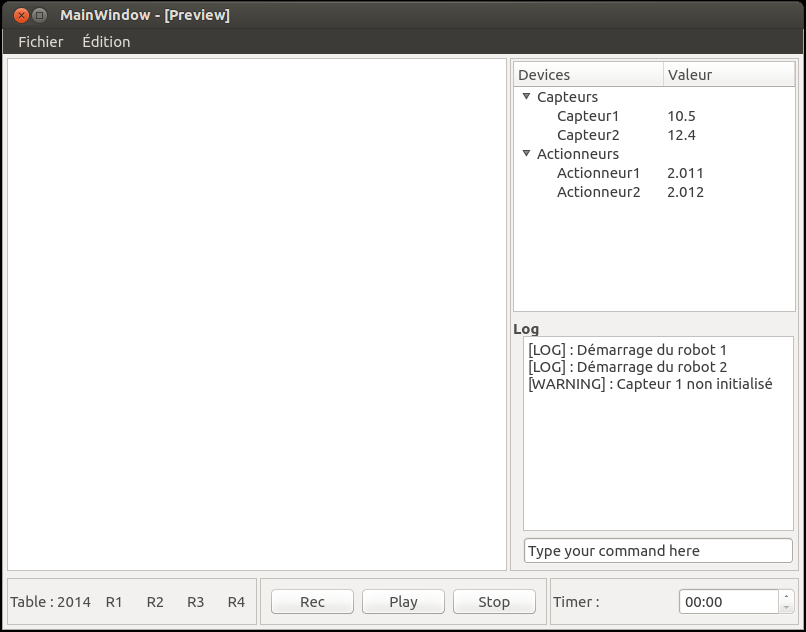
\includegraphics[scale=0.5]{GUI.png}
\vspace{5 mm}
\\

Cette interface devra proposer les fonctionnalités suivantes : 

\subsection{Besoins fonctionnels}

\subsubsection{Arborescence des onglets fichier et édition}
\textbf{Fichier}
\begin{itemize}
\item Nouveau
\item Ouvrir
\item Enregistrer sous
\item Enregistrer
\end{itemize}

\textbf{\'Edition}
\begin{itemize}
\item Insertion
    \begin{itemize}
    \item Objet
    \item Erreur $\rightarrow$ Choix du capteur ou de l'actionneur et de la nouvelle Valeur
%%    \item 
%%    \item 
    \end{itemize}

\item Table
\begin{itemize}
\item {Choix du Fichier de Description $\rightarrow$ Choix de l'Année} \footnote{"$\rightarrow$" signifie qu'une fenêtre s'ouvre pour réaliser l'action}
\end{itemize}
\item Supprimer Table

\item Ajouter un robot
    \begin{itemize}
    \item Robot 1 $\rightarrow$ Choix du fichier de description
    \item Robot 2 $\rightarrow$ Choix du fichier de description
    \item Robot 3 $\rightarrow$ Choix du fichier de description
    \item Robot 4 $\rightarrow$ Choix du fichier de description
    \end{itemize}
\item Supprimer Robot ( une fenêtre s'ouvre pour le choix des robots à supprimer )
%\item 
\end{itemize}

% \textbf{Affichage}
% \begin{itemize}
% \item Insertion
%     \end{itemize}
% \begin{itemize}
% \item Ajouter un robot
    
%\end{itemize}

\subsubsection{Afficher l'environnement en 2D vu du dessus}
%N ET T
Afin de suivre facilement l'avancement de la simulation, l'utilisateur doit avoir un retour visuel simple de la simulation. Le but de cet affichage est de proposer une vue pertinante concernant les déplacements des robots sur la table en fonction des objectifs. Les actions de ramassage d'objets ne sont pas simulées précisément et ne nécessitent donc pas de vue en 3D.
La vue en 2D du dessus est donc la plus adaptée ici. Elle sera agrémentée d'informations telles qu'une coloration spécifique du robot en fonction de l'équipe, une mise en valeure des objectifs selon l'équipe.

\subsubsection{Afficher la trace récente de l'exécution}
%N ET T
En cas de comportement non voulu l'utilisateur doit avoir un retour précis des valeurs des modules, ainsi que des messages échangés à travers le socket correpondant. une trace de cette exécution doit donc s'afficher dans le cadre \texttt{log} à droite de la vue 2D. Ces logs réunissent les erreurs d'éxecutions tels que les overflows, les warnings, et tous les messages entre le robot et le simulateur (les actions sur les actionneurs et les capteurs, ainsi que les erreurs simulées).

\subsubsection{Choisir les paramètres d'exécution de la simulation}
%N ET T
Avant de commencer la simulation l'utilisateur peut sélectionner un/des robots, tables parmi ceux configurés par les fichiers de description importés.
Celui-ci peut ensuite préciser une position initiale pour chaque robot choisi.
Après avoir sélectionné ses paramètres, l'utilisateur pourra lancer la simulaion avec le bouton "play".

Il sera possible d'enregistrer la simulation au fur et à mesure de son exécution avec le bouton "record". La manière d'enregistrer cette exécution est précisée dans le chapitre dédié au simulateur.

Au lieu de charger les paramètres tel que décrit ci-dessus, il peut être possible de charger une simulation préalablement enregistrée et la rejouer.


\subsubsection{Pendant la simulation}
%N ET T
Une fois la simulation lancée, il doit être possible de la mettre en pause afin de mieux analyser les valeurs retournées par les capteurs à un instant t, et également avoir la possibilité de changer à la volée les valeurs retournées de manière à tester la robustesse du comportement du robot face à des données erronnées.
De plus, l'utilisateur doit pouvoir intéragir directement avec la simulation quand elle est en pause afin d'amener des perturbations. Il sera possible d'insérer un élément, un robot ou une erreur à l'aide de l'option \texttt{Insérer} de l'onglet \texttt{\'Editer}.









\newpage
\section{Langage de description}
%TODO 
% relire et changer pargraphe représentation selon commentaires !
Pour pouvoir répondre aux signaux de l'exécutable, le simulateur doit savoir où, quoi et comment regarder. Donc, il faut mettre en place un langage de description des robots et de l'environnement.

\label{langdesc}

\subsection{Description des Robots}

\label{desc_robot}

Les robots sont des objets complexes et modifiés chaque année. Il est donc impératif d'avoir un langage facile à maitriser, modifier et ce, sans connaissance du fonctionnement du simulateur. Il devra spécifier où sont placés les actionneurs et autres capteurs. Leur position doit être fournie dans le repère cartésien centré sur le barycentre du robot et son angle de rotation propre (rotation autour de la verticale). Lorsque l'utilisateur questionne l'élément il doit pouvoir renvoyer son état. Pour ce faire, il interrogera la bibliothèque dynamique contenant la spécification de chaque capteurs. Le langage doit aussi spécifier si une partie du robot est mobile, ainsi que son degré de mobilité. En outre, chacun de ces éléments doit être identifié de manière unique pour permettre à l'exécutable d'appeler l'objet en question. Ce lien est fournit par la broche sur laquelle vient se brancher cet élément. Enfin, pour répondre aux critères de simplicité, la description du robot se fera selon le schéma de descritpion XML en annexe \ref{descbot}.

\subsection{Description de la Table}

La table est la partie majoritaire de la simulation. C'est l'environnement sur lequel se déplacent les robots. Elle possède des parties fixes, généralement composées de formes géométriques simples, et des parties mobiles. La table nécessite donc aussi une description avec le placement de ses parties mobiles à l'initialisation. Le fichier de description doit donc contenir ces informations ainsi que la nature de l'élément de jeu concerné. Sa forme, sa position de départ mais aussi son poid nécessaire à la simulation. De même que pour les Robots, la description sera en XML et respectera le fichier de descritpion en annexe \ref{desctable}.

\subsection{Représentation}

% Cette phrase n'est pas claire 
% par description est-ce tu veux dire fichier de description ? si oui quel   % format ?
% interpréter les demandes de l'exécutable, oui mais lequel ? exécutable     % robot ?
% moteur physique soit capable de fournir les données demandées. 
% Ok mais les fournir à qui ? pourquoi ?

% c'est mieu? JR
Chacun de ces éléments doit avoir une description telle que présentée dans le paragraphe précédent pour pouvoir paramétrer le moteur physque.
Ainsi qu'une représentation en 3 dimensions pour que ce dernier soit capable de fournir les données demandées par les modules de la bibliothèque dynamique. 

Il faut donc utiliser un système de maillage compréhensible par le moteur physique et par l'interface utilisateur qui en fera une projection dans le plan de la table. Les formes de la table sont toujours simples mais celles des robots peuvent être assez rapidement compliquées. C'est pourquoi le format de mesh doit pouvoir être exporté d'un logiciel de dessin ou de CAO tel que Blender ou Autodesk Inventor.

%% ldauphin
Le format de description de maillage qui semble le plus simple et supporté en export par tout les logiciels de CAO est le format STL (STereoLithographie). Le simulateur devra donc parser ce format pour le transformer en données compréhensibles par le moteur physique. 

%% ldauphin
Ce format permet de définir plusieurs objets solides par leurs faces, elles mêmes déterminées par des points dans l'espace. Il peut être textuel ou binaire. Nous supporterons dans un premier temps uniquement le format textuel.

Voici un exemple de fichier STL :

\begin{verbatim}
solid name

    facet normal ni nj nk
        outer loop
            vertex v1x v1y v1z
            vertex v2x v2y v2z
            vertex v3x v3y v3z
            ...
        endloop
    endfacet
    
    ...

endsolid name
\end{verbatim}

\newpage
\section{Bibliothèque de composants}
%% Clément : je pense que c'est mieux tourné de cette manière, je travaille encore dessus

Les bibliothèques dynamiques simulant chacune un module physique des robots (actionneur, capteur) sont à la charge de l'utilisateur. Néanmoins, SASIAE sera fourni avec quelques modules de base ainsi que la documentation nécessaire pour implémenter de nouveaux modules.

Chacune de ces bibliothèques dynamiques seront, de part l'utilisation du framework Qt, des plugins qui pourront dont aisément s'intégrer dans le reste de l'application. Nous utiliserons donc la classe QPluginLoader que nous instancierons autant de fois que de types de module sont nécessaires.

Un plugin représente bien un type de module et non un module seul car un robot voire même les robots simulés peuvent embarquer plusieurs fois le même composant. Le plugin contiendra évidement le code permettant la simulation du composant mais surtout, en tant qu'objet principale, une fabrique permettant d'instancier le dit composant et d'obtenir quelques informations à son sujet.

De part le besoin de généraliser le processus d'instanciation et d'utilisation d'un composant, la fabrique ainsi que la classe simulant un composant respecteront toutes deux des interfaces bien définies et seront ces dernières qui seront également bien documentées, permettant ainsi au client de créer de nouveaux composants dans le futur de manière aisée. (\`A noter qu'un développement supplémentaire dans Aversive++ sera certainement également nécessaire pour apporter une abstraction de ce nouveau composant au code robot)

La fabrique respectera l'interface \emph{ModuleFab} suivante (encore incomplète/à discuter) :
\begin{itemize}
    \item Module* create(const QMap\textless QString, QVariant\textgreater \&) const : permet d'instancier un module avec les paramètres donnés dans la QMap
    \item QString name() const : retourne le nom du module correspondant
    \item ...
\end{itemize}

Tandis que les modules respecteront l'interface \emph{Module} suivante (de même) :
\begin{itemize}
    \item $[$slot$]$ refresh() \emph{(paramètres à réfléchir)} : permet de rafraichir le module après qu'un pas de simulation ait été calculé
    \item $[$signal$]$ message(QString) : permet d'ajouter un message dans le journal/log
    \item $[$signal$]$ hasChanged(const Module*) : permet d'informer que le module à changer d'état (permettant de mettre à jour l'UI et envoyer le nouvel état à l'API du code robot correspondant)
    \item const QSharedPointer / QMap\textless QString, QVariant\textgreater\ \emph{(à réfléchir)} data() const : permet de récupérer la/les valeurs du composant
    \item ...
\end{itemize}

%benoit
%Tous les modules de la bibliothèque ont une classe dans l'api, le dialogue entre code robot (via API) et le module de la bibliothèque ce fait par message text voir %TODO ref%
%.

%Le coordinateur dialogue avec les modules par 4 méthode défini dans la classe abstraite moduleDynamique, qui sont :
%\begin{itemize}
%    \item{Constructeur(CoordinateurModule *)} : permet de donner au  module l'objet a contacter.
%    \item{apiMessage(const char* s)} : donne un message de la part du code robot.
%    \item{simulStep(btDiscreteDynamicsWorld* world)} : indique qu'un pas de simulation a été calculé, et qu'il faut le transformer en donnée pour le code robot. Le pas de simulation suivant ne sera pas calculer tant que tous les modules n'auront pas fini leurs simulStep.
%\end{itemize}

%Dans l'autre sens, defini par l'interface CoordinateurModule:
%\begin{itemize}
%    \item{send()} : envoie d'un message text à l'API
%    \item{valeurCapteur<type t>(t valeur)} : valeur d'un capteur a retressetre a l'utilisateur et au robot.
    %\item{done()} : indique au coordinateur que le module a fini son traitement et qu'un nouveau pas de simulation peut commencer.
%    \item{bulletAdd(btRigidBody* objet)} indique au coordinateur d'ajouter un objet dans la scene.
%\end{itemize}

%Les modules ne communique pas a proprement parler au moteur physique, ils ont juste access au objets de la simulation via une pointeur et a leurs propriété modifié au cours la simulation.
%Un capteur de distance pourra par exemple crée son propre rayTest pour calculer la distance de son module à l'obstacle suivant.


\newpage
\section{Architecture}
%%%% Clément %%%%
\label{architecture}

Le développement de l'application sera découpé en plusieurs parties :
\begin{itemize}
    \item le GUI se chargera de l'interaction avec l'utilisateur ;
    \item le moteur physique s'occupera de simuler l'environnement physique ;
    \item le coordinateur s'occupera :
    \begin{itemize}
        \item de charger les bibliothèques dynamiques simulant les différents modules physiques et mécaniques ;
        \item d'interpréter le fichier de description de la table pour la charger dans le moteur physique ;
        \item d'interpréter le fichier de description d'un robot pour le modéliser dans le moteur physique, de lancer son ou ses exécutables, d'établir la communication avec les processus ainsi créés et d'instancier les différents modules nécessaires pour ce robot ;
        \item de journaliser certains évenements de la simulation ;
    \end{itemize}
\end{itemize}

Aversive++, implémentation\_simulation sera, quant à elle, linkée lors de la compilation avec le code robot et elle s'occupera de la communication avec le coordinateur.

Elle comportera un \texttt{Client} "de coordination" qui s'occupera de récupérer les messages du coordinateur de manière asynchrone par rapport au code robot, mettre à jour les données de capteurs, ainsi que gérer l'execution des tâches enregistrées dans les schedulers (voir partie\ref{planif_taches} Planification des tâches) .

Au sein de l'application :
\begin{itemize}
    \item le GUI communiquera avec le coordinateur et le moteur physique pour récupérer et afficher une vue de l'environnement physique, la ou les valeurs des capteurs et afficher le journal de la simulation ;
    \item le coordinateur et le moteur physique intéragiront ensemble afin que les différents modules puissent calculer leurs valeurs (dans le cas de capteurs) ou modifier des valeurs (dans le cas d'actionneur) ;
\end{itemize}

%%%%%%%%%%%%%%%%%%%%%%%%%%%%%%%%%%%%%%%%%%%%%%%%%%%%%%%%%%%%%%%%%%%%%%%%%%%%%%%
%%% Je touve les deux figure redondantes et la secondes est plus complète et plus agréable à regarder. JR
%%% +1 (Loïc)

%\vspace{5 mm}
%\begin{figure}
%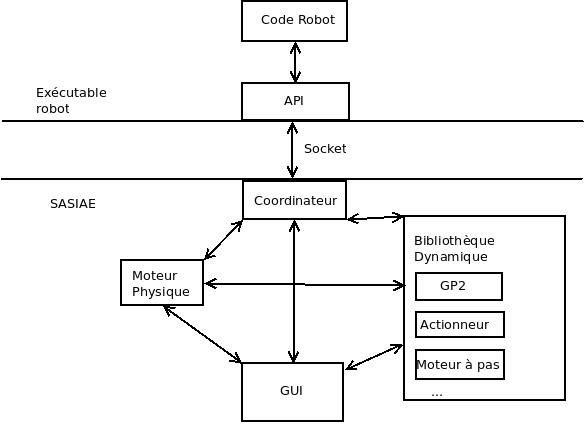
\includegraphics[scale=0.80]{architecture.png}
%\caption{shéma de l'architecture globale de SASIAE}
%\label{figurearchitecture}
%\end{figure}
%\vspace{5 mm}

%\newpage

La figure \ref{messagearchitecture} présente de façon un peu plus détaillée les messages envoyés entre les différents composants du simulateur.
L'objet "Module" est un module générique qui peut être un capteur et un actionneur, il y aura dans l'application plusieurs modules, mais le schéma 
n'en comporte qu'un pour des soucis de lisibilité.

%% Clément : C'est quoi ce "ClientCoordination" côté exécutable robot qui reçoit les valeurs des capteurs ? C'est Aversive++ qui est aussi censé gérer et fournir une abstraction des capteurs !!!

\begin{figure}
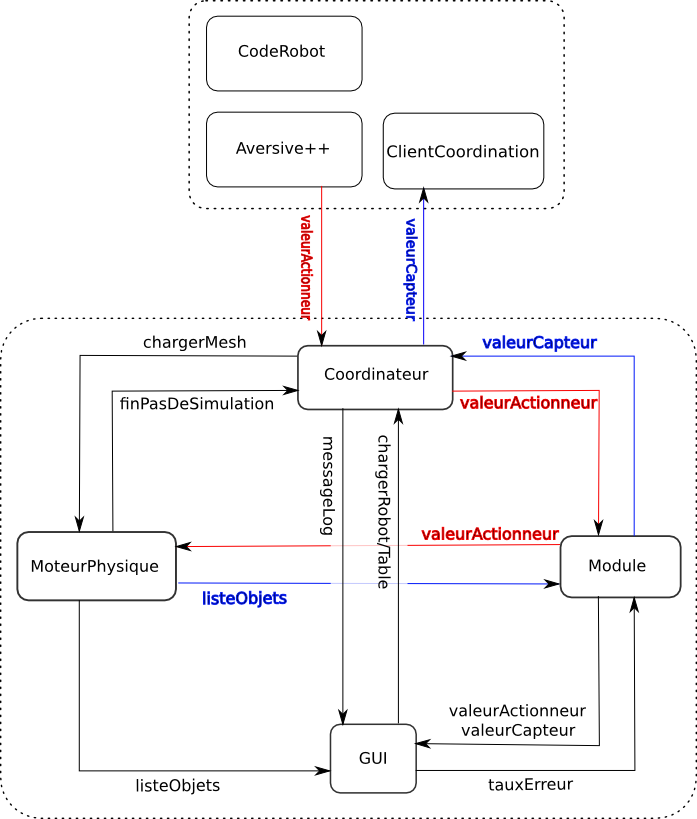
\includegraphics[scale=0.70]{architecturemsg.png}
\caption{messages entre les composants de l'architecture}
\label{messagearchitecture}
\end{figure}
\vspace{5 mm}

\newpage
%%benoit :
\section{Communication entre l'exécutable robot et le logiciel de simulation}

Le code du robot doit être un exécutable indépendant du logiciel de simulation, cet exécutable robot doit être produit par une simple compilation en utilisant la partie spécifique simulation de l'API Aversive++. Finalement, ces deux exécutables, celui du code robot et celui du logiciel, doivent communiquer ensemble.

\subsection{Moyen de communication}

%Hugo
La communication entre le logiciel de simulation et l'exécutable robot
doit être bidirectionnelle. Cela permet à l'exécutable robot d'envoyer
des ordres aux actionneurs, et des messages à l'utilisateur. Ou dans
l'autre sens, la simulation peut transmettre la valeur des différents
capteurs simulés à l'exécutable robot, tout comme elle peut simuler un module
interne au microcontrôleur (Horloge, UART, Analogic to Digital
Converter, ports). Ces modules dépendent fortement du micro-contrôleur
utilisé. Ces messages ne sont pas synchrone et
n'attendent aucune réponse.
%HUGO : Vérifier qu'on parle bien qlqpart dans le cahier des charges 
% du fait qu'on importe en bibliothèque dynamique tout les modules
% nécessaire, c'est-à-dire leur émulation.
% Clément: bien précisé dans bibliotheque.tex je pense ;)

Pour que les deux exécutables puissent identifier les objets auxquels
ils parlent, ils utilisent le port utilisé dans le cas d'une ressource
externe au microcontrôleur (branchée sur une/des pins de la carte donc), ou bien le nom de cette ressource si elle est interne au microcontrôleur. % interne à quoi ? 
Dans le cas où l'exécutable du robot envoie sur un port des
données ne correspondant pas aux valeurs attendu par le coordinateur,
un message d'erreur est envoyé à l'utilisateur.


Pour faire la communication, on utilise un socket dans lequels on envoie des messages séparés par des sauts de lignes le tous codé en ANSI.
%quel format de fichier pour ces messages ? 
\subsection{Syncronisation simulation - exécution robot}

Pour indiquer au code robot qu'il peut faire des calculs, c'est à dire
qu'un pas de simulation est à faire coté robot, un message de
synchronisation est envoyé.

%% Clément : wut? je veux dire, on simule simplement le module timer du microcontrolleur que le scheduler utilisera et ça devrait être aussi simple que cela puisque le robot devrait être bloqué dans un while(1) le reste du temps
%% (Loïc) Sauf que le wile(1) sera pas vide. Du moins pas forcément.

\subsection{Detail des messages échangeables}
Les messages doivent contenir les champs suivant :
\begin{itemize}
    \item{Type de message :}
    \begin{itemize}
        \item{Texte pour l'utilisateur}
        \item{Message d'un module}
        \item{Valeur d'un capteur / actionneur}
        \item{Synchronisation}
    \end{itemize}
\end{itemize}

Dans le cas des messages texte à l'intention de l'utilisateur :
\begin{itemize}
    \item{Le type de message :}
    \begin{itemize}
        \item{Info}
        \item{Warning}
        \item{Error}
    \end{itemize}
    \item{Le message texte :}
    \begin{itemize}
        \item{Le texte en une seule ligne}
    \end{itemize}
\end{itemize}

Dans le cas des valeurs d'un objet :
\begin{itemize}
    \item{Identificateur de l'objet :}
    \begin{itemize}
        \item{pins auquelles il est branché.}
    \end{itemize}
    \item{Types des valeurs : (peut etre un tableau à deux dimension de valeurs)}
    \begin{itemize}
        \item{Nombre de lignes}
        \item{Type de la première colonne (parmi bool, int, float, charactère)}
        \item{Type de la deuxième colonne}
        \item{...}
    \end{itemize}
    \item{Valeurs}
    \begin{itemize}
        \item{Séparées par des virgules}
        \item{Avec les chaines de caractères entre double-quotes}
    \end{itemize}
\end{itemize}

Message de module :
\begin{itemize}
    \item{Type de l'objet}
    \begin{itemize}
        \item{doit correspondre au nom d'un module dynamique}
    \end{itemize}
    \item{Identificateur de l'objet}
    \begin{itemize}
        \item{pins dans le cas d'un module externe au microcontroleur}
        \item{nom de la ressource pour les modules internes au microcontroleur}
    \end{itemize}
    \item{Chaine de caractères à destination du module dynamique gérant le périphérique}
\end{itemize}

Pour les initialisations, c'est un message de module contenant la chaine de caractère INIT, suivit des paramètres séparé par des espaces.

Pour les messages de syncronisation deux type de message :
\begin{itemize}
    \item{Nouveau pas de simulations}
    \item{Code robot en attente}
\end{itemize}



\newpage
\chapter{Conclusion}

\section{Validation de l'application}
%% Les étapes qui permettrons de dire que le contrat est remplis
Ici sont listés les différents livrables à produire en cours de projet :

%\begin{enumerate}
    \subsubsection{Première série de livrables}
    \begin{itemize}
    
        \item{La fenêtre principale de l'application, décrite plus haut, et dont une image a été montrée.}
        
        \item{Une première version d'Aversive++ minimale permettant de coder avec les actionneurs et capteurs suivants : Encodeur, Moteurs de propulsion, gestion des tâches.\\ Les interfaces implémenteront la communication avec le simulateur et des tests permettront de vérifier cette communication.}

        \item{Un environnement physique minimal gérant un robot (codé en dur) se déplaçant sur une table plane et permettant de modifier la vitesse de ses moteurs.}
        
        \item{Les modules encodeur et moteur.}
        
    \end{itemize}
    \subsubsection{Deuxième série de livrables}
    \begin{itemize}
        
        \item{Le coordinateur minimal permettant l'interaction entre le code robot et modules.}
        
        \item{Complétion de l'API avec : GP2, AX12, Servomoteur, Balise de détection, gestion des overflows.}
        
        \item{Ajout des modules GP2, AX12, Servomoteur, Balise de détection.}
        
    \end{itemize}
    \subsubsection{Troisième série de livrables}
    \begin{itemize}
        
        \item{L'intégration du moteur physique au coordinateur.}
        
        \item{Introduction des erreurs dans le retour de capteurs et dans l'execution des commandes par les actionneurs.}
        
        \item{L'environnement physique complet, avec plusieurs robots, et une table chargeable.}
        
    \end{itemize}
    \subsubsection{Quatrième série de livrables}
    \begin{itemize}
        
        \item{Complétion du coordinateur pour qu'il puisse charger dynamiquement les modules en mémoire et rediriger les ordres vers les modules adéquats.}
        
        \item{Afficher l'environnement de la table avec les robots sur la fenêtre principale, ainsi que la valeur des capteurs et le log de tous les évènements.}
        
        \item{La partie de l'interface graphique permettant de charger des fichiers de configurations.}
        
        \item{Le coordinateur permettant plusieurs robots dans le scénario. Il doit aussi permettre de charger les robots, la table depuis un fichier, et uniquement les modules utilisés par les robots.}
        
    \end{itemize}
    \subsubsection{Derniers livrables}
    \begin{itemize}
        
        \item{Pouvoir placer les robots sur la table en début de simulation depuis l'interface graphique.}
        
        \item{Les interfaces de l'API, et les modules de simulateur associés pour tous les actionneurs/capteurs suivants : UART, I2C, Lidar.}
        
    \end{itemize}
%\end{enumerate}

\section{Évolution envisagées}
%%\begin{itemize}

%%% (ldauphin) : je les ait placé dans validation : voir le main.tex pour explication de la raison + cours de Génie Logiciel
%%% Je les garde au cas ou j'ai oublié quelque chose

%%\item{Premier incrément :}
%%GUI: affiche 2D de la scène, la valeur des capteurs et des messages de log et démarage de la simulation.
%%Moteur physique : interaction avec le coordinateur et le GUI.
%%Coordinateur : table et robot codé en dur, communication avec le robot et les modules.
%%modules API: timer, gp2, moteur et roue codeuse.
%%modules simulation: timer, gp2, moteur et roue codeuse.

%%\item{Deuxieme incrément :}
%%les autres modules (uart, i2c, servomoteur, ax12), mode pause/resume dans la simulation, ajout d'obstacle.

%%\item{Troisième incrément :}
%%Charger les donnés de la table et du robot (plus codé en dur), erreur des capteurs.

%%\item{Dernier incrément :}
%%Prendre en compte l'ensemble des pièces et leurs caractéristiques (matérieux, masse, coeficient d'adérence), tous les actionneurs du robot %%dans la simulation (via le moteur physique) et leurs interactions avec l'environement (servomoteur, moteur pas à pas ...).
%%\end{itemize}

Liste des améliorations à apporter au projet :
\begin{itemize}
	\item{Ajout d'un éditeur de table.}
	\item{Ajout d'un éditeur de robot.}
	\item{Avoir l'affichage de la simulation en 3D.}
	\item{Mise en place des règles de jeux avec calcul des scores.}		
	\item{Ajout d'un fonctionnement temps réel avec le robot branché (type Hardware-in-the-loop) incluant le réglage automatique des paramètres d'asservissement.}
	\item{Génération de code à partir de l'interface graphique.}
\end{itemize}


%% ce qu'on a envie de faire, mais qu'on aurai pas le temps

\section{Planning}
\begin{tabular}{rp{8cm}|p{3cm}}

    2 décembre 2013 &&\\
    
    %2
    &
    La fenêtre principale de l'application &
    Nicolas, Théotime \\
    
    &&\\
    
    %2
    &
    Première version d'Aversive++ minimale &
    Loïc, Clément \\
    
    &&\\
    
    %2
    &
    Environnement physique minimal &
    Jean-Raymond, Hugo \\
    
    &&\\
    
    %1
    &
    Les modules encodeur et moteur &
    Benoît \\
    
    23 décembre 2013 &&\\
    
    %3
    &
    Intéraction entre le code robot et modules &
    Clément, Benoît, Hugo \\
    
    &&\\
    
    %2
    &
    Modules GP2, AX12, Servomoteur, Balise de détection &
    Loïc, Théotime \\
    
    &&\\
    
    %2
    &
    Complétion d'Aversive++ avec les interfaces GP2, AX12, Servomoteur, Balise de détection &
    Jean-Raymond, Nicolas\\

    27 javier 2014 &&\\

    %3
    &
    Intégration du moteur physique au coordinateur &
    Loïc, Nicolas, Jean-Raymond \\
    
    &&\\
    
    %2
    &
    Introduction des erreurs &
    Théotime, Hugo \\
    
    &&\\
    
    %2
    &
    L'environnement physique complet &
    Clément, Benôit \\
    
    10 février 2014 &&\\
    
    %2
    &
    Charger dynamiquement les modules en mémoire &
    Théotime, Benoît \\
    
    &&\\
    
    %2
    &
    Afficher l'environnement sur la fenêtre principale &
    Loïc, Hugo \\
    
    &&\\
    
    %1
    &
    Charger des fichiers de configurations (gui) &
    Jean-Raymond \\
    
    &&\\
    
    %2
    &
    Le coordinateur permettant plusieurs robots &
    Clément, Nicolas \\
    
    3 mars 2014 &&\\
    
    %3
    &
    Pouvoir placer les robots sur la table &
    Théotime, Benoït, Hugo \\
    
    &&\\
    
    %4 (2 aversive + 2 modules)
    &
    UART, I2C, Lidar (Aversive++ et modules) &
    Loïc, Clément, Nicolas, Jean-Raymond \\
    
    24 mars 2014 &&\\
    
    &
    Rendu final &
    \\
    
\end{tabular}


\newpage
\section{Annexes}
\subsection{Format XML}
\subsubsection{Descritpion d'un robot}
\begin{changemargin}{-1cm}{-1cm}
\begin{lstlisting}[caption=Description du Robot, label=descbot]
<?xml version="1.0" encoding="UTF-8"?>
<xs:schema
        xmlns:xs="http://www.w3.org/2001/XMLSchema">
    <xs:element name="robot">
    <xs:complexType>
        <xs:sequence>
            <xs:element name="mesh">
            <xs:complexType>
                <xs:attribute name="src" type="xs:string"/>
            </xs:complexType>
            </xs:element>
            <xs:element name="microcontroller">
            <xs:complexType>
                <xs:sequence>
                    <xs:element name="modules">
                    <xs:complexType>
                        <xs:sequence>
                            <xs:element name="module">
                            <xs:complexType>
                                <xs:sequence>
                                    <xs:element name="location" minOccurs="0" maxOccurs="xs:unbounded">
                                    <xs:complexType>
                                        <xs:attribute name="X" type="xs:Integer"/>
                                        <xs:attribute name="Y" type="xs:Integer"/>
                                        <xs:attribute name="Z" type="xs:Integer"/>
                                        <xs:attribute name="alpha">
                                            <xs:restriction base="xs:integer">
                                                <xs:minInclusive value="0"/>
                                                <xs:maxInclusive value="360"/>
                                            </xs:restriction> 
                                        </xs:attribute>
                                        <xs:attribute name="beta">
                                            <xs:restriction base="xs:integer">
                                                <xs:minInclusive value="0"/>
                                                <xs:maxInclusive value="360"/>
                                            </xs:restriction>
                                        </xs:attribute>
                                        <xs:attribute name="gamma">
                                            <xs:restriction base="xs:integer">
                                                <xs:minInclusive value="0"/>
                                                <xs:maxInclusive value="360"/>
                                            </xs:restriction>
                                        </xs:attribute>
                                    </xs:complexType>
                                    </xs:element>
                                    <xs:element name="parameters">
                                    <xs:complexType>
                                        <xs:sequence>
                                            <xs:element name="parameter" minOccurs="0" maxOccurs="xs:unbounded">
                                                <xs:complexType>
                                                    <xs:attribute name="name" type="xs:String" use="required"/>
                                                    <xs:attribute name="type" type="xs:String" use="required"/>
                                                    <xs:attribute name="value" type="xs:String" use="required"/>
                                                </xs:complexType>
                                            </xs:element>
                                        </xs:sequence>
                                    </xs:complexType>
                                    </xs:element>
                                </xs:sequence>
				<xs:attribute name="name" type="xs:string"/>
                            </xs:complexType>
                            </xs:element>
                        </xs:sequence>
                    </xs:complexType>
                    </xs:element>
                </xs:sequence>
	        <xs:attribute name="name" type="xs:string"/>
            </xs:complexType>
            </xs:element>
        </xs:sequence>
    </xs:complexType>
  </xs:element>
</xs:schema>
  \end{lstlisting}
\end{changemargin}

\subsubsection{Exemple de Robot}
\begin{lstlisting}[caption=Exemple de Robot, label=exrobot]
<robot>
	<mesh src="~/mesh/robots/robot1A1314.stl"/>
	<microcontroller name="UNIOC">
		<modules>
			<module name="GP2">
				<location X="10" Y="-2" Z="10" alpha="0" beta="0" gamma"0"/>
				<parameters>
                                	<parameter name="bell" type="int" value="20"/>
				</parameters>
			</module>
		</modules>
	</microcontroller>
</robot>
\end{lstlisting}
  
\clearpage
\subsubsection{Description de la Table}
 \begin{lstlisting}[caption=Description de la Table, label=desctable]
<?xml version="1.0" encoding="UTF-8"?>
<xs:schema
        xmlns:xs="http://www.w3.org/2001/XMLSchema">
    <xs:element name="table">
    <xs:complexType>
        <xs:sequence>
            <xs:element name="mesh">
                <xs:attribute name="src" type="xs:string">
            </xs:element>
            <xs:element name="toys">
            <xs:complexType>
                <xs:sequence>
                    <xs:element name="toy">
                    <xs:complexType>
                        <xs:attribute name="weight" type="xs:integer"/>
                        <xs:attribute name="name" type="xs:string"/>
                        <xs:sequence>
                            <xs:element name="location" minOccurs="1" maxOccurs="xs:unbounded">
                            <xs:complexType>
				<xs:attribute name="X" type="xs:Integer"/>
				<xs:attribute name="Y" type="xs:Integer"/>
				<xs:attribute name="Z" type="xs:Integer"/>
				<xs:attribute name="alpha">
				    <xs:restriction base="xs:integer">
					<xs:minInclusive value="0"/>
					<xs:maxInclusive value="360"/>
				    </xs:restriction> 
				</xs:attribute>
				<xs:attribute name="beta">
				    <xs:restriction base="xs:integer">
					<xs:minInclusive value="0"/>
					<xs:maxInclusive value="360"/>
				    </xs:restriction>
				</xs:attribute>
                                <xs:attribute name="gamma">
				    <xs:restriction base="xs:integer">
					<xs:minInclusive value="0"/>
					<xs:maxInclusive value="360"/>
				    <xs:restriction>
				</xs:attribute>
			    </xs:complexType>
			    </xs:element>
			    <xs:element name="mesh">
			    <xs:complexType>
				<xs:attribute name="src" type="xs:string">
			    </xs:complexType>
			    </xs:element>
                        </xs:sequence>
                    </xs:complexType>
                    </xs:element>
                </xs:sequence>
            </xs:complexType>
            </xs:element>
	</xs:sequence>
    </xs:complexType>
</xs:element>
\end{lstlisting}
  
\subsubsection{Exemple de Table}
\begin{lstlisting}[caption=Exemple de table, label=desctable]
<table>
    <mesh src="~/mesh/table/t1314.stl"/>
	<toys>
	    <toy name="triangle1" weight="170">
		<location X="10" Y="10" Z="10" alpha="0" beta="0" gamma="0"/>
		<mesh src="~/mesh/jouets/triangle1314.stl"/>
	    </toy>
	</toys>
</table>
\end{lstlisting}




\end{document}
